% This is an example of using latex for a paper/report of specified
% size/layout. It's useful if you want to provide a PDF that looks
% like it was made in a normal word processor.

% While writing, don't stop for errors
\nonstopmode

% Use the article doc class, with an 11 pt basic font size
\documentclass[11pt, a4paper]{article}

% Makes the main font Nimbus Roman, a Times New Roman lookalike:
%\usepackage{mathptmx}% http://ctan.org/pkg/mathptmx
% OR use this for proper Times New Roman (from msttcorefonts package
% on Ubuntu). Use xelatex instead of pdflatex to compile:
\usepackage{fontspec}
\usepackage{xltxtra}
\usepackage{xunicode}
\defaultfontfeatures{Scale=MatchLowercase,Mapping=tex-text}
\setmainfont{Times New Roman}

% Nice citations
\usepackage{natbib}

% Set margins
\usepackage[margin=2.5cm]{geometry}

% Multilingual support
\usepackage[english]{babel}

% Nice mathematics
\usepackage{amsmath}

% Left right harpoons for kinetic equations
\usepackage{mathtools}

% Control over maketitle
\usepackage{titling}

% Section styling
\usepackage{titlesec}

% Ability to use colour in text
\usepackage[usenames]{color}

% For the \degree symbol
\usepackage{gensymb}

% Allow includegraphics and nice wrapped figures
\usepackage{graphicx}
\usepackage{wrapfig}
\usepackage[outercaption]{sidecap}
\usepackage{subfigure}

% Nice quotes
\usepackage{csquotes}

% Set formats using titlesec
\titleformat*{\section}{\bfseries\rmfamily}
\titleformat*{\subsection}{\bfseries\itshape\rmfamily}

% thetitle is the number of the section. This sets the distance from
% the number to the section text.
\titlelabel{\thetitle.\hskip0.3em\relax}

% Set title spacing with titlesec, too.  The first {1.0ex plus .2ex
% minus .7ex} sets the spacing above the section title. The second
% {-1.0ex plus 0.2ex} sets the spacing the section title to the
% paragraph.
\titlespacing{\section}{0pc}{1.0ex plus .2ex minus .7ex}{-1.1ex plus 0.2ex}

%% Trick to define a language alias and permit language = {en} in the .bib file.
% From: http://tex.stackexchange.com/questions/199254/babel-define-language-synonym
\usepackage{letltxmacro}
\LetLtxMacro{\ORIGselectlanguage}{\selectlanguage}
\makeatletter
\DeclareRobustCommand{\selectlanguage}[1]{%
  \@ifundefined{alias@\string#1}
    {\ORIGselectlanguage{#1}}
    {\begingroup\edef\x{\endgroup
       \noexpand\ORIGselectlanguage{\@nameuse{alias@#1}}}\x}%
}
\newcommand{\definelanguagealias}[2]{%
  \@namedef{alias@#1}{#2}%
}
\makeatother
\definelanguagealias{en}{english}
\definelanguagealias{eng}{english}
%% End language alias trick

%% Any aliases here
\newcommand{\mb}[1]{\mathbf{#1}} % this won't work?
% Emphasis and bold.
\newcommand{\e}{\emph}
\newcommand{\code}[1]{\textsf{#1}}
\newcommand{\dvrg}{\nabla\vcdot\nabla}
%% END aliases

% Custom font defs
% fontsize is \fontsize{fontsize}{linespacesize}
\def\authorListFont{\fontsize{11}{11} }
\def\corrAuthorFont{\fontsize{10}{10} }
\def\affiliationListFont{\fontsize{11}{11}\itshape }
\def\titleFont{\fontsize{14}{11} \bfseries }
\def\textFont{\fontsize{11}{11} }
\def\sectionHdrFont{\fontsize{11}{11}\bfseries}
\def\bibFont{\fontsize{10}{10} }
\def\captionFont{\fontsize{10}{10} }

% Caption font size to be small.
\usepackage[font=small,labelfont=bf]{caption}

% Make a dot for the dot product, call it vcdot for 'vector calculus
% dot'. Bigger than \cdot, smaller than \bullet.
\makeatletter
\newcommand*\vcdot{\mathpalette\vcdot@{.35}}
\newcommand*\vcdot@[2]{\mathbin{\vcenter{\hbox{\scalebox{#2}{$\m@th#1\bullet$}}}}}
\makeatother

\def\firstAuthorLast{James}

% Affiliations
\def\Address{\\
\affiliationListFont Adaptive Behaviour Research Group, Department of Psychology,
  The University of Sheffield, Sheffield, UK \\
}

% The Corresponding Author should be marked with an asterisk. Provide
% the exact contact address (this time including street name and city
% zip code) and email of the corresponding author
\def\corrAuthor{Seb James}
\def\corrAddress{Department of Psychology, The University of Sheffield,
  Western Bank, Sheffield, S10 2TP, UK}
\def\corrEmail{seb.james@sheffield.ac.uk}

% Figure out the font for the author list..
\def\Authors{\authorListFont Sebastian~S.~James, Stuart~P.~Wilson  \Address \\
  \corrAuthorFont $^{*}$ Correspondence: \corrEmail}

% No page numbering please
\pagenumbering{gobble}

% A trick to get the bibliography to show up with 1. 2. etc in place
% of [1], [2] etc.:
\makeatletter
\renewcommand\@biblabel[1]{#1.}
\makeatother

% reduce separation between bibliography items if not using natbib:
\let\OLDthebibliography\thebibliography
\renewcommand\thebibliography[1]{
  \OLDthebibliography{#1}
  \setlength{\parskip}{0pt}
  \setlength{\itemsep}{0pt plus 0.3ex}
}

% Set correct font for bibliography (doesn't work yet)
%\renewcommand*{\bibfont}{\bibFont}

% No paragraph indenting to match the VPH format
\setlength{\parindent}{0pt}

% Skip a line after paragraphs
\setlength{\parskip}{0.5\baselineskip}
\onecolumn

% titling definitions
\pretitle{\begin{center}\titleFont}
\posttitle{\par\end{center}\vskip 0em}
\preauthor{ % Fonts are set within \Authors
        \vspace{-1.1cm} % Bring authors up towards title
        \begin{center}
        \begin{tabular}[t]{c}
}
\postauthor{\end{tabular}\par\end{center}}

% Define title, empty date and authors
\title {
%  Competition can account for stopping in a gradient-following model
%  of the retinotectal projection \\
%  \emph{or} \\
%  Competition provides stopping for the chemoaffinity
%  theory which is robust to noise \\
%  \emph{or} \\
%  Self-organisation of topographically ordered axon connections can take place
%  in a noisy environment if axons compete \\
%  \emph{or} \\
Time to stop; agent-based modelling of chemoaffinity with competition
}
\date{} % No date please
\author{\Authors}

% Simplified chemoaffinity explains retinotectal mapping via local axon-axon
% interactions
%
% Focus on the chemoaffinity idea for this model. Show that local interactions
% can provide an account for growth cones finding their targets.

%% END OF PREAMBLE

\begin{document}

\setlength{\droptitle}{-1.8cm} % move the title up a suitable amount
\maketitle

\vspace{-1.8cm} % HACK bring the introduction up towards the title. It
                % would be better to do this with titling in \maketitle

% Note this is the SfN draft abstract, and will need rewriting.
\emph{In the classic Chemoaffinity theory, the retinotectal axon projection is
thought to use pairs of orthogonal signalling gradients in the retina to
specify the eventual location of synapses made on the surface of the
tectum/superior colliculus. Similar orthogonal gradients in the tectum provide
a coordinate system which allows the axons to match their prespecified
destination with the correct location. Although the Ephrins have been shown to
guide axons toward their destination, there has yet to emerge a complete
account of the local interactions which halt the axonal growth cones in the
correct locations to recreate the topography of the retinal cells. The model
of \citet{simpson_simple_2011} provides an account of the basic topographic
arrangement of cells on the tectum, as well as reproducing well known surgical
and genetic manipulation experiments. However, it suffers from the absence of
a local chemotactic guidance mechanism. Instead, each agent in that model is
given instantaneous knowledge of the vector that would move it toward its
pre-specified destination. In addition to the globally supervised
chemoaffinity term, \citet{simpson_simple_2011} introduced a competitive
interaction for space between growth cone agents and a receptor-receptor
axon-axon interaction in order to account for the full set of experimental
manipulations. Here, we propose the replacement of the chemoaffinity term with
a gradient following model consisting of axonal growth cone agents which carry
receptor molecule expression determined by their soma's location of origin on
the retina. Growth cones move on the simulated tectum guided by two pairs of
opposing, orthogonal signalling molecules representing the Ephrin ligands. We
show that with only the receptor-ligand mediated chemoaffinity term and a
receptor-receptor based axon-axon interaction term (meaning that all growth
cone interactions are communicated by receptor signalling), a full range of
experimental manipulations to the retinotectal system can be
reproduced. Furthermore, we show that the observation that competition is not
an essential requirement for axons to find their
way \citep{gosse_retinotopic_2008} is also accounted for by the model, due to
the opposing influences of signalling gradient pairs. Finally, we demonstrate
that, assuming exponentially varying receptor expression in the retina, tectal
ligand expression should either be exponential if the receptor-ligand signal
induces repulsion (i.e. gradient descent) or logarithmic if the signal induces
attraction (gradient ascent). Thus, we find that a model analogous to the one
we presented in \citet{james_modelling_2020} that accounts for murine barrel
patterning is also a candidate mechanism for the arrangement of the more
continuous retinotectal system.}

%%%%%%%%%%%%%%%%%%%%%%%%%%%%%%%%%%%%%%%%%%%%%%%%%%%%%%%%%%%%%%%%%%%%%%%%%%%%%%%
\section{Introduction}

The retinotectal projection has been an important model system in the study of
how the cells of the central nervous system are accurately connected together
into functional networks. This projection connects the light-gathering cells
in the retina to movement-related cells in the optic tectum (known as the
superior colliculus in mammals). Light sources originating close to each other
in the environment tend to activate retinal ganglion cells (either
directly \cite{iRGC_citation} or indirectly via rods and cones) situated close
together in the eye so that an image of the environment is formed on the
retinal surface. It has been discovered that the topography of the retina is
preserved within brain regions that process this information such that cells
which are adjacent within the retina primarily excite cells adjacent in the
tectum. This indicates that during development there must exist a mechanism
which ensures the correct arrangement of the axons which leave the retina and
connect to cells in the tectum.

One reason for the success of the study of the retinotectal projection is its
capacity to be experimentally manipulated. In some non-mammalian species, both
the retina and the tectum can be partially ablated, or even physically
reorganised in-vivo, after which axons regrow to restore the order and
function of the system for the individual animal. This manipulability was
exploited in influential work by R. W. Sperry and co-workers during the
mid-twentieth century, leading to Sperry's 1963 summary of
the \emph{chemoaffinity theory} \citep{sperry_chemoaffinity_1963} which
proposes the existence of morphogenetic gradients that guide axons to their
destination. The chemoaffinity theory was given robust support by the
discovery of the ephrin ligands and their receptors \citep{cheng_complementary_1995,drescher_vitro_1995}
which have been shown to form into graded expression fields in the
retina \citep{braisted_graded_1997}, tectum \citep{braisted_graded_1997,feldheim_genetic_2000} as well as in other
sensory systems, such as the somatosensory
system \citep{vanderhaeghen_mapping_2000}. The Ephrin ligands have a clear
effect on axonal outgrowth, as shown in in-vitro \citep{cheng_complementary_1995,drescher_vitro_1995,hansen_retinal_2004} and
in-vivo \citep{frisen_ephrin-a5_1998,rodger_transient_2000,mann_topographic_2002,hindges_ephb_2002} studies.
%
% A-P:
%
% EphA and ephrinAs: Anteroposterior axis of retiontectal projection
% (Nasal-Temporal on retina; Anteroposterior on tectum).
%
% RGM (tectum) Neogenin (retina)
%
% D-V:
%
% EphB and ephrin B: Dorsoventral on retina; dorsoventral on tectum.
%
% En-2: Repels temporal growth cones of xenopus ret-tec axons and attracts
% nasal ones. Brunet et all, Nature, 2005
%
% Ryk/Fz (retina) and Wnt3 (tectum) (Flanahan, 2006)
%

It is tempting to consider the retinotectal projection well understood. With a
comprehensive theory supported by a biochemical mechanism, is there anything
left to understand? That question can be answered by reviewing retinotectal
modelling papers.

Mini-review here, which contrasts some of the modelling papers. The upshot is
that a central problem with models is not how the axons know how to get closer
to their destination, but how they know they have \emph{arrived} at their true
destination. Also make the point that many of the models are phenomenological
in nature and do not elucidate the mechanisms behind the arrangement.

In a recent paper, we proposed a self-organising mechanism, based on
morphogenetic signalling gradients, which can arrange
axons growing from the thalamus to the somatosensory cortex into the well
known murine barrel cortex pattern~\citep{james_modelling_2020}. In
characterising that system, we explored the effect of various types of
noise. We found that the mechanism was robust to noise in the expression of
the signalling molecules over a wide range of amplitudes and length-scales,
and that noise in the interaction parameters, which are obtained by sampling
the signalling molecules in the source tissue (the thalamic barreloid field)
could cause topological defects. The question of noise in axon guidance has
been explored by \citet{goodhill_can_2016}.

\textbf{New introduction:} Simpson and Goodhill presented a model in which the
chemoaffinity mechanism is non-biological. We offer a model in which a
competition mechanism counteracts the drive of axons along the ephrin
gradient. Will we need the axon-axon interaction mechanism based on
non-same-Eph repulsion?

\textbf{Another approach:} We present a model of gradient-following based on graded
interactions between the growth cones of retinal ganglion cell axons and the
tectal surface. We show that a combination of exponentially graded expression
in the retina \citep{reber_relative_2004} and exponentially (for repulsively
interacting receptor ligand pairs) \emph{or} logarithmically (for attractively
interacting receptor/ligands) graded expression on the tectum permits a purely
local model to reproduce the majority of reported phenomena associated with
retinotectal organisation.

There have been many approaches to modelling the organisation of the
retinotectal projection. Many of these models are wholly or partially
phenomenological.

A model which carefully deals with receptor
binding is given by \citet{naoki_revisiting_2017} \citep[see also][]{mortimer_bayesian_2009}.

Gradient based models: \citet{nakamoto_topographically_1996}

\section{Model}

Our model was inspired by the agent-based model of \cite{simpson_simple_2011}
and, in common with that work, consists of agents representing axonal growth
cones, originating from a square retina and moving upon a square tectum of
side length 1 in arbitrary units.
%
\citet{simpson_simple_2011} model three contributions to the movement of the growth
cones; chemoaffinity, competition for space and axon-axon interactions. The
first two of these are modelled without reference to a particular mechanism;
each agent is provided with globally-supervised information about its
instantaneous location and its target location, allowing it to move along a
vector towards the target. Competition is implemented as a movement of
constant distance along the vector between two agents if those two agents are
within a threshold distance of one another. Interaction is signal-induced
repulsion, which is triggered if two agents are both within the threshold
distance of each other and have compatible EphA receptor expression.

We sought to replace the globally-supervised mechanisms by local receptor and
ligand based interactions. First, chemoaffinity was remodelled so that all
interactions occurred via signal transmission between the receptors expressed
on the growth cones of retinal ganglion cell axons and the ligands expressed
across the tectum. Signals induced either an attractive or repulsive
interaction to cause growth cones to ascend or descend the gradient of ligand
expression on the tectum.

We then explored the behaviour of models incorporating this chemoaffinity
mechanism alone and in conjunction with several competition mechanisms. We
found parameters for the best models of each type (chemo-only [G],
chemo-competition [GC], chemo-receptor-receptor [GI] and chemo-receptor-ligand
[GJ]) by an optimisation approach. We then compared each model's ability to
reproduce the surgical and genetic manipulation results in a manner similar to
that taken by \citet{simpson_simple_2011} to find the simplest model that
would fit the data.

\subsection*{Receptor and ligand expression}

\begin{figure}
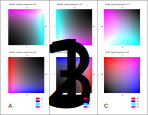
\includegraphics[width=\linewidth]{./images/expressions_fig.png}
\caption{Simulated retinal and tectal signalling molecule expression. Four
receptor types are expressed, and four corresponding ligand types. Receptors
of type $i$ are activated by ligands of type $i$.
%
\textbf{A} Retinal receptor expression, $r_i$. Four receptors are expressed and
displayed here in two dual-colour maps. $r_0$ and $r_1$ are red and blue;
$r_2$ and $r_3$ are cyan and magenta. $r_0$ increases as an exponential
function of $-x$; $r_1$ increases with an exponential function of $-y$. $r_2$
and $r_3$ have the opposite sense. Retinal receptor expression is modelled
with exponential functions because there is ample evidence to support this
form. $N$: nasal, $T$: temporal, $D$: dorsal, $V$: ventral.
%
\textbf{B} Retinal ligand expression, $l_i$, is expressed in complimentary
gradients \citep{hornberger_modulation_1999}.
%
\textbf{C} Tectal ligand expression $L_i$. Tectal ligand expression is shown in a linear form,
as there is less evidence to determine whether ligand expression is
exponential, linear or logarithmic on the tectum.
$L$: lateral, $M$: medial, $C$: caudal, $R$: rostral.
}
\label{f:ex}
\end{figure}

Each retinal ganglion cell projects $n$ growth cone agents (referred to
as \emph{branches}) which carry a set of 4 receptors, $r_i$, and 4 ligands,
$l_i$, indexed by $i$ and expressed at levels determined by the cell's
location on the retina. The expression levels of the receptors and ligands
vary with respect to the cell's position on the retinal surface. Each receptor
or ligand varies only with respect to one dimension.  Receptor expression
gradients are arranged in orthogonal pairs with the gradient of $r_0$ being
orthogonal to that of $r_1$. $r_2$, whose gradient is opposite to $r_0$, is
orthogonal to $r_3$. Ligands are also arranged in orthogonal pairs, with $l_0$
opposing $r_0$ (as $r_0$ increases, $l_0$ decreases) and $l_1$ orthogonal to
$l_0$ and opposing $r_1$.

Because there is convincing evidence that EphA and EphB receptors are
expressed in exponentially increasing
patterns \citep{reber_relative_2004,feldheim_genetic_2000,brown_topographic_2000,koulakov_stochastic_2004},
we use an exponential form for retinal receptor expressions, in common with
other modelling
studies~\citep{reber_relative_2004,koulakov_stochastic_2004,simpson_simple_2011}.
We adopt the same precise form for the retinal receptor expression
as \citet{simpson_simple_2011} which is
\begin{equation} \label{e:retrcpt}
r_i(x,y) = 1.05 + 0.26 \exp(2.3 x)
\end{equation}

The simulated tectum expresses the same types of receptors and ligands, also
in orthogonal pairs of gradients. In this work, we did not consider the effect
of reverse signalling from tectal receptors to RGC ligands so we only modelled
tectal ligand expression, $L_i$. Although several studies model tectal ligand
expression with exponential functions \citep{koulakov_stochastic_2004}, the
experimental evidence for ligand expression is more ambiguous (Supp. Fig
\textbf{X}). Correspondingly, we leave open the possibility that tectal ligand
expression may be modelled by exponential, linear or logarithmic functions:
\begin{equation} \label{e:tecligexp}
L_i^{\text{exp}}(x,y) = 1.05 + 0.26 \exp(2.3 x)
\end{equation}
or
\begin{equation}
L_i^{\text{lin}}(x,y) = 1.31 + 2.33 x;
\end{equation}
or
\begin{equation}
L_i^{\text{log}}(x,y) = 2.32 + 1.29 \log (2.3(x+0.2))
\end{equation}
Each function has approximately the same expression values at $x=0$ and
$x=1$. Opposing functions are obtained by substituting $(1-x)$ for $x$.

While we do not explicitly name $r_0$, $r_1$,
etc.~as \emph{EphA}, \emph{EphB}, the suggestion is that $r$ includes EphA,
EphB, Ryk \citep{schmitt_wntryk_2006} and
Neogenin \citep{rajagopalan_neogenin_2004} receptors and that $l$ and $L$
include the ephrin-A, ephrin-B, Wnt3 \citep{schmitt_wntryk_2006} and
RGM \citep{monnier_rgm_2002} ligands, each of which has been shown to play a
role in retinotectal map formation.

Figure~\ref{f:ex} shows colour maps of receptor and ligand expression, in this
case tectal ligand expression maps are linear. Note that the expression is
discretized, and in simulations, the gradient is computed numerically from the
discretized expression. This makes it straightforward to perform tectal and
retinal `graft' manipulations. Coordinates within the simulated retina and
tectum are normalised, with 1 corresponding to 2 mm on the tectum and on the
retina for mouse \citep{reber_relative_2004}. This means that growth cones of
approximate radius 5 $\mu$m = 0.005 mm \citep{goodhill_can_2016} have a
radius $r$ = 0.0025 in the arbitrary units of the simulation. For a realistic
simulation based on mouse, the approximate RGC density in the retina is around
44000 cells per retina \citep{jeon_major_1998}. This sets the side length of
the retina to $\sqrt{44000} \approx 200$. This results in a simulation of
prodigious computational size, which although tractable (10 s per step,
requiring several hours, rather than days to run) is not convenient. To
maintain the relationship between growth cone size and cell density, we permit
a smaller number of growth cones ($400\times8=3200$) but keep the fractional
area of the branches at 0.86 ($44000 \times \pi r^2$) (if there is one cone
per axon) or 6.9 (if there are 8 cones per axon).

\subsection*{Movement}

At each timestep in a simulation, the position, $\mathbf{x}_{b,t}$, at time
$t$ of each branch $b$ is updated according to
%
\begin{equation}
\mathbf{x}_{b,t+1} = \mathbf{x}_{b,t} + \mathbf{M}_{b}
\end{equation}
%
where $\mathbf{M}_{b}$, the movement vector, is the sum of a chemoaffinity
effect, $\mathbf{G}_b$, axon-axon competition, $\mathbf{C}_b$, an axon-axon
receptor-receptor interaction, $\mathbf{I}_b$, and axon-axon receptor-ligand
interaction, $\mathbf{J}_b$, and a `border effect',
$\mathbf{B}_b$, which acts to retain branches within the tectal region:
%
\begin{equation}
\mathbf{M}_{b} = m_1 \mathbf{G}_b + m_2 \mathbf{C}_b + m_3 \mathbf{I}_b +
m_4 \mathbf{J}_b + m_5 \mathbf{B}_b
\end{equation}
%
evaluated at time $t$. $m_1$--$m_5$ are scalar parameters. We typically
considered models for which some of $m_2$ to $m_4$ were fixed to zero. A model
for which $m_3$ and $m_4$ were zero was named a `$\mathbf{GC}$' model as it
combined the chemoaffinity effect and space-based competition; a model for
which $m_2$ was zero was a `$\mathbf{GIJ}$' model and so on.

\subsection*{Chemoaffinity}

In this model, the signal transmitted when a ligand binds to a receptor on a
branch (forward signalling) can lead to one of two effects; the signal may
induce an attraction towards the ligand-expressing region or a repulsion away
from it.
%
For axon-tectum interactions, we implemented attraction as a climbing of the
tectal ligand expression gradient and repulsion as gradient descent.
%
To determine the strength of the effect we assumed a purely linear receptor
binding model, and set the chemotactic movement vector of the branch $b$ at
location $\mathbf{x}_b$ on the tectum to be
%
\begin{equation}
\mathbf{G}_b = \sum_i^N F_i\,r_{i,b} \nabla L_i(\mathbf{x}_b)
\end{equation}
%
where $r_{i,b}$ is the receptor expression on branch $b$ for ligand-receptor
pair $i$, $\nabla L_i$ is the gradient of expression of ligand $i$ on the
tectum and $F_i$ denotes the direction of the interaction induced when a
molecule of ligand $i$ binds to a receptor $i$ molecule. $F_i$ takes the value
-1 for a repulsive interaction or 1 for an attractive interaction.

\subsection*{Axon-axon interactions}

We investigated three forms of competition that could be combined with the
chemoaffinity effect. We investigated space-based competition
(`$\mathbf{C}$'), as described in \citet{simpson_simple_2011}, a
receptor-receptor signalling mechanism (`$\mathbf{I}$'), similar to that
described in \citet{simpson_simple_2011}, and a receptor-ligand mass-action
signalling model (`$\mathbf{J}$'). Our aim was to determine whether either of
the receptor/ligand based signalling mechanisms could replace the space-based
competition.

\subsection*{Space based (or self-other) competition}

Space based competition is a repulsive effect which acts between any two
branches, whether they originate from different retinal ganglion cells or from
the same cell. It assumes that there is some kind of self-other signal which
acts to discourage two cells from approaching each other.
%
\begin{equation}
\mathbf{C}_b = \frac{1}{|B_{b,c}|} \sum_k \hat{\mathbf{x}}_{kb} W
\end{equation}
where the distance based weight $W$ is given by
\begin{equation}
W_c(d_{kb}) = \begin{cases}
      1 - \frac{d_{kb}}{2r_c}   & d_{kb} \leq 2r_c \\
     0 & d_{kb} > 2r_c
     \end{cases}
\end{equation}
for two growth cones of interaction radius $r_c$ separated by a distance
$d_{kb}$. $B_{b,c}$ is the set of growth cones within a distance $2r_c$ of
branch $b$.

\subsection*{Receptor-receptor axon-axon interactions}

We modelled interactions between axon growth cones due to signalling between
receptors of the same type. For these interactions, repulsion caused a
movement of branch $b$ along a unit vector, $\hat{\mathbf{x}}_{kb}$, from
branch $k$ to branch $b$ causing them to move further apart; attraction caused
the opposite movement. This interaction, $\mathbf{I}_b$, acting on branch $b$,
is given by
%
\begin{equation}
\mathbf{I}_b
= \frac{1}{|B_{b,I}|} \sum_k \sum_i \hat{\mathbf{x}}_{kb}\,W_I \qquad \mathrm{if}~r_{i,b}
/ r_{i,k} < 1.1
\end{equation}
%
the weight here is defined as a function of $r_I$:
%
\begin{equation}
W_I(d_{kb}) = \begin{cases}
      1 - \frac{d_{kb}}{2r_I}   & d_{kb} \leq 2r_I \\
     0 & d_{kb} > 2r_I
     \end{cases}
\end{equation}
$r_{i,k}$ is the expression of receptor $i$ on branch $k$.

\subsection*{Receptor-ligand axon-axon interactions}

%
\begin{equation}
% No \frac{1}{|B_b|} in this one. Really?
\mathbf{J}_b = \sum_k \hat{\mathbf{x}}_{kb}\,Q_J(d_{kb})
\end{equation}
%
where $Q_J(d_{kb})$ is the signalling strength between two growth cones of
receptor-ligand interaction radius $r_j$ a distance $d_{kb}$ from one another,
given by
%
\begin{equation}
Q_J(d_{kb}) = \begin{cases}
     \sum_i^N F_i\,r_{i,b}\,l_{i,k}    & d_{kb} \leq 2r_j \\
     0 & d_{kb} > 2r_j
     \end{cases}
\end{equation}
%
The sign of $Q_J$ (which is dependent on the values of $F_i$) determines whether
the interaction, $\mathbf{I}_b$, is repulsive or attractive. $l_{i,k}$ is the
expression of ligand $i$ on branch $k$.

\subsection*{Border effect}

We implemented a border effect based on gradient following by assuming that
there is some other molecular signal which acts on all branches near the
boundary of the tectal tissue. For a branch with position $(x,y)$, $\mathbf{B}_b$ is
given by:
%
\begin{equation}
B_{b,x} = \begin{cases}
        r-x      & x<r \\
        1-r-x    & x>1-r
\end{cases}
B_{b,y} = \begin{cases}
        r-y      & y<r \\
        1-r-y    & y>1-r
\end{cases}
\end{equation}
%
Thus $\mathbf{B}_b$ is equivalent to the action of a repulsive signalling
molecule expressed around the border of the tectum, whose expression increases
quadratically outside the tectum and affects any branch touching (or outside)
the boundary

\subsection*{Initial conditions}

Branches were randomly distributed in a stripe at the rostral side of the
tectum at the start of each simulation. Each RGC axon was assigned a random
initial position coordinate:
\begin{equation}
\mathbf{x}_{\text{axon},t=0} = (U(0,1), U(-0.2,0))
\end{equation}
where U(p,q) is a number selected from a random uniform distribution in the
range $[p,q)$. Each of the $n$ branches per RGC axon was given its parent
axon's initial position, plus a randomly generated offset with coordinates
derived from a normal distribution of mean 0 and standard deviation 0.1.

\subsection*{Assumptions}

% All the extra bits of info required to specify the simulation
To enable a simulation of the model described above it is necessary to make
some assumptions about the nature of the receptor-ligand signalled
interactions (i.e. the values of $F_i$ that determine whether interactions are
attractive or repulsive) and about the pattern of ligand expression on the
tectal surface. Unless stated otherwise, we assumed that: \textbf{i)} all
receptor-ligand signalled interactions are repulsive ($F_i=-1, \forall i$), as
for EphA-ephrinA
coupling \citep{drescher_vitro_1995,nakamoto_topographically_1996};
and \textbf{ii)} all tectal ligand expressions vary exponentially along a
given axis, following Eq.\,\ref{e:tecligexp}.

In all simulations, the border effect, $B_b$, had the same magnitude with
$m_5=0.5$. The number of branches per axon was 4 unless otherwise stated.

\section{Results}

\subsection*{Chemoaffinity as the sole patterning mechanism}

The first question we tried to answer was whether chemoaffinity alone,
implemented as gradient following, is sufficient to pattern the tectum. We set
$m_1=0.002$ and $m_2=m_3=m_4=0$ and ran the model for 300
steps.

Results are shown in Fig.\,\ref{f:ch}. Fig.\,\ref{f:ch}A indicates the colour
code used for retinal cell position; dorsal retinal cells are indicated by
green, nasal cells by red. Lightness gives position along the relevant axis so
that cells at the dorsal-nasal corner are yellow and those at the
ventral-transverse corner are black. Fig.\,\ref{f:ch}E shows the expected
layout of retinal ganglion cell axons on the tectum. The axons retain the
colour of their originating cell on the retina, as shown in
Fig.\,\ref{f:ch}A. Nasal cell axons should be arranged caudally; dorsal axons
laterally; axons should be evenly spaced and the pattern should span the
entire tectum.  Fig.\,\ref{f:ch}B--D show `fish net' plots of the axon
centroids at three timepoints. An axon's centroid is the average location of
its 4 branches. In these plots, lines are drawn between axons that are
expected to arrange themselves adjacently to one another by the end of the
simulation. The number of line crossings in this plot gives an indication of
the disorder in the arrangement. Fig.\,\ref{f:ch}G shows the positions of the
individual branches (i.e.~growth cones) at $t=300$ that contribute to the the
plot in Fig.\,\ref{f:ch}D. By this time, the topological order matches that
shown in Fig.\,\ref{f:ch}E. Opposing gradients have sorted the axons along the
two axes to form a grid of cells. However, the arrangement does not span the
full tectum. Fig.\,\ref{f:ch}F shows two pattern metrics; the sum of squared
distance errors of the axon centroids and the number of crossings in the fish
net plot of Fig.\,\ref{f:ch}D. The expected number of crossings is 0, as in
Fig.\,\ref{f:ch}E. Fig.\,\ref{f:ch}H shows selected axons (one from the centre
and one from each corner of the retina) and their position history.

% ./build/sim/agent/agent1 configs/simpler/m_ee_G.json configs/simpler/e_wt_fig2.json
\begin{figure}
\includegraphics[width=\linewidth]{./images/j4_ee_G_wt_fig2.png}
\caption{The pure gradient-following model.}
\label{f:ch}
\end{figure}

The form of the retinal receptor expression (Eq.\,\ref{e:retrcpt}) is based on
empirical measurement, but the tectal ligand expression
(Eq.\,\ref{e:tecligexp}) was chosen arbitrarily. To expand the pattern in
Fig.\,\ref{f:ch}D so that it covers the entire tectum, we needed only to
adjust the tectal ligand expression, substituting the alternative exponential
expression:
%
\begin{equation} \label{e:tecligexp2}
L_i^{\text{exp}}(x,y) = 1.05 + 0.26 \exp(1.1 x)
\end{equation}

for the tectal ligand expression.

The result at $t=300$ is shown in Fig.\,\ref{f:chalt}A and B. The axon
centroids are arranged across the full tectal surface.  The arrangement is
slightly disordered around the middle of the tectum. This is caused by
numerical artefacts from the discretization of the ligand expression and the
fact that in the centre, the difference between the opposing receptor-ligand
signals is very small. Nevertheless, it is demonstrated that a modified form
for the tectal ligand expression (which was found easily by hand tuning)
allows a well ordered map to form for the wildtype system. Fig
.\,\ref{f:chalt}C shows the error metric, which is closer to 0 with the new
ligand expression.

% ./build/sim/agent/agent1 configs/simpler/m_eE_G.json  configs/simpler/e_wt_fig2.json
\begin{figure}
\includegraphics[width=\linewidth]{./images/j4_eE_G_wt_fig3.png}
\caption{The pure gradient-following model (alt exponential).}
\label{f:chalt}
\end{figure}

The `chemoaffinity only' model begins to encounter problems when we introduce
simulations of experimental manipulations.

% The chemo manipulations figure is made up from 4 figures generated with graph_layout::?
\begin{figure}

\includegraphics[width=\linewidth]{./images/fig_chemo_manipulations.png}
\caption{Surgical manipulations in the chemoaffinity-only model. Row A: wildtype. Row B: 90 degree
rotation. Row C: 180 degree rotation. Row D: Graft swap}
\label{f:chsurg}
\end{figure}

\subsection*{Normal development}

To enable a simulation it is necessary to make assumptions about the nature of
the receptor-ligand signalled interactions (i.e. whether they are attractive
or repulsive) and about the pattern of ligand expression on the tectal
surface. We assume that i) All receptor-ligand signalled interactions are
repulsive, as for EphA-ephrinA
coupling \citep{drescher_vitro_1995,nakamoto_topographically_1996}; and ii)
all tectal ligand expressions vary exponentially along a given axis, following
Eq.\,\ref{e:tecligexp}. The results of running such a system are presented in
Fig.\,\ref{f:wt}.
%
Fig.\,\ref{f:wt}Ai shows a dual-colour map of retinal ganglion cell positions
on the square retina, with red encoding position on the $x$ axis (temporal to
nasal) and green encoding position on the $y$ axis (ventral to
dorsal). Fig.\,\ref{f:wt}Aii presents a fishnet plot of the expected location on
the tectal surface of each RGC at the end of the development process. Thus,
the `red' RGC from the ventro-nasal corner should map to the caudo-medial
corner of the tectum and the `green' RGC from the dorso-temporal corner should
find its way to the rostro-lateral corner on the tectum. The lines between the
dots of Fig.\,\ref{f:wt}Aii indicate the adjacency relationships between
cells. Thus, colour in each panel indicates a branch or axon's location of
origin on the retina.
%
Fig.\,\ref{f:wt}B shows the initial state of the system, with branches
stochastically arranged around the rostral edge of the tectum. Each dot
represents the centroid of $n=8$ branches per RGC axon. Figs.\,\ref{f:wt}C and \ref{f:wt}D
show the development of the system with time, with Fig.\,\ref{f:wt}D showing a
well ordered arrangement, with a majority of adjacency relationships matching
the experimental prediction (i.e. there are few crossed lines). The
intermediate timepoint at $t=40$ indicates that branches quickly cover the simulated
tectal surface, with final adjacency relationships developing over a longer
timescale. This dynamic behaviour is also evident in Fig.\,\ref{f:wt}E, which
shows \textbf{RMS error or some metric} of the axon centroids with respect to
the experimental prediction. Fig.\,\ref{f:wt}F shows the final
location of each branch in the simulation, which gives a more continuous view
of the order present in Fig.\,\ref{f:wt}D. Finally, Fig.\,\ref{f:wt}G shows the
branches and their centroid path history for five selected RGCs, with path
histories strongly resembling those presented by \citet{simpson_simple_2011}.

This result shows that a gradient-following model based on receptor-ligand
interactions (both for axon-to-tectum and axon-to-axon interactions) is
able to generate the basic mapping observed in the retinotectal projection.

\subsection*{Manipulations}

To determine if the model can explain the many surgical and genetic
manipulations described in the literature
\citep*[for a review, see][]{goodhill_retinotectal_1999} we performed
simulations matching those in \citet{simpson_simple_2011} in which we either
rotated or translocated grafts of the tectum; ablated portions of the retina
and/or the tectum; or manipulated the receptor or ligand expressions in the
model.

\subsubsection*{Surgical Manipulations}

Fig.\,\ref{f:surg1} shows the result of simulating three surgical
manipulations alongside the wildtype result, which is shown on Row A. Rows B
and C show graft rotation simulations (90$\degree$ and 180$\degree$). In each
case an 8x8 square on the tectum (each unit is 0.05x0.05) is rotated. The
rotational sense can be observed clearly in the `Branches' column; for the
90$\degree$ rotation, the top-right (caudal-lateral) corner of the rotated
square is red, whereas the top-left corner of the wildtype tectum is red. \textbf{etc}.


%
\includegraphics[width=\linewidth]{./images/fig_manipulations.png}

\begin{figure}
\begin{subfigure}{\linewidth}
\includegraphics[width=\linewidth]{./images/j4_eE_GJ_wt_rotcmp.png}
\end{subfigure}
\begin{subfigure}{\linewidth}
\includegraphics[width=\linewidth]{./images/j4_eE_GJ_tecrot90.png}
\end{subfigure}
\begin{subfigure}{\linewidth}
\includegraphics[width=\linewidth]{./images/j4_eE_GJ_tecrot180.png}
\end{subfigure}
\begin{subfigure}{\linewidth}
\includegraphics[width=\linewidth]{./images/j4_eE_GJ_tecswap.png}
\end{subfigure}
\caption{Surgical manipulations. Row A: wildtype. Row B: 90 degree
rotation. Row C: 180 degree rotation. Row D: Graft swap.}
\label{f:surg1}
\end{figure}

Fig.\,\ref{f:surg2} shows retinal ablation, tectal ablation, mismatch and
compound eye experiments (Stuart: see Simpson and Goodhill Fig. 4).

\begin{figure}
\begin{subfigure}{\linewidth}
\includegraphics[width=\linewidth]{./images/j4_eE_GJ_retablate.png}
\end{subfigure}
\begin{subfigure}{\linewidth}
\includegraphics[width=\linewidth]{./images/j4_eE_GJ_tecablate.png}
\end{subfigure}
\begin{subfigure}{\linewidth}
\includegraphics[width=\linewidth]{./images/j4_eE_GJ_mismatch.png}
\end{subfigure}
\begin{subfigure}{\linewidth}
\includegraphics[width=\linewidth]{./images/j4_eE_GJ_compound.png}
\end{subfigure}
\caption{Surgical manipulations 2. Row A: Retinal ablation, Row B: Tectal
ablation, Row C: Mismatch (ablate retina and also the tectum that matches the
left-behind retina), Row D: Compound eye (Two nasal retinal halves `glued
together')}
\label{f:surg2}
\end{figure}

\subsubsection*{Genetic manipulations}

Brown et al. EphA knock-in.

\begin{figure}
\includegraphics[width=\linewidth]{./images/j4_ee_brown.png}
\caption{Brown et al simulation. This is EphA3 knockin - it adds a constant to
half of the RGC's $r_0$ (randomly selected). Compare with S\&G Fig.\,6.}
\label{f:brown}
\end{figure}

Describe Reber and other gene knock-in and knock-out experiments.

\begin{figure}
\includegraphics[width=\linewidth]{./images/j4_ee_reber.png}
\caption{Reber et al simulation. Follow on to Brown et al (same
group). Combines the selective EphA3 knockin with a uniform EphA4 knockdown.}
\label{f:reber}
\end{figure}

\subsection*{ligand expression profiles}

A section to show the effect of assuming linear or logarithmic expression
profiles. Especially that linear expression fails to reproduce the rotation
and graft swap manipulations. Hmm, actually, it looks ok?!

\subsection*{Attractive receptor-ligand interactions}

Show that, if you switch one of the receptor-ligand  interactions in the
system to be attractive instead of repulsive, then you have to make the ligand
expression form logarithmic instead of exponential.

\begin{figure}
\includegraphics[width=\linewidth]{./images/j4_ee_ephb_wt.png}
\caption{The effect of making one interaction attractive. This models
switching one receptor/ligand pair to be an analogue of EphB, but retains an
assumption that the ephrin-B ligand has exponential form. The change compared
with the model of Fig.\,\ref{f:wt} is that the tectal ligand direction of
$L_1$ is reversed and the interaction of $r_1$ and $L_1$/$l_1$ is made
attractive. $L_1$ retains the assumption of exponential change. Note the
`bunching up' of the field to the medial side of the tectal sheet.}
\label{f:ee_oneattractive}
\end{figure}

\begin{figure}
\includegraphics[width=\linewidth]{./images/j4_eel_ephb_wt.png}
\caption{The arrangement is restored by making the expression of $L_1$ on the
tectal sheet change logarithmically.}
\label{f:eel_oneattractive}
\end{figure}

\subsection*{Grating simulations}

I'd like to do this if it's not too much work!

\section{Discussion}

The model described above assumes that branches express graded levels of
receptors which interact with ligands expressed as gradients on the tectum,
the tectal border and on the surface of other branches, and that only these
interactions guide their movement.

\subsection*{Results Observations/Notes}

J has a repulsive effect, which is generally disordering. If competition has
`a lot of work to do' (i.e. in the m\_ee... models) then a strong J will push
the axons across the whole tissue, but will upset the local ordering
relationships. Perhaps J also needs a self-self interaction (i.e. for members
of the same axon?).

The I interaction is absent when the topographic ordering is good. This means
that it does not fix the retablate condition. Like the other competition
effects, it is strongly affected by the radius of interaction.


% Discuss the Hill Equation! https://en.wikipedia.org/wiki/Hill_equation_(biochemistry)
% This relates to the work \cite{naoki_revisiting_2017}

%
% BIBLIOGRAPHY
%
\selectlanguage{English}
\bibliographystyle{apalike}
\bibliography{RetinoTectal}

\end{document}


%% For the noise based paper:
%% Instead, we treat the receptor binding at the growth cone with greater
%% care. Based on a Michaelis-Menten model applied to
%% receptor binding, \citet{mortimer_bayesian_2009} give an expression for the
%% probability of an individual receptor being bound as a function of the ligand
%% expression, $\gamma$, and the ligand gradient, $\mu$;
%% \begin{equation}
%% P(b=1|\gamma,\mu) = \frac{\gamma(1 + \mu r)}{1 + \gamma(1 + \mu r)},
%% \end{equation}
%% where $r$ is the distance of the receptor from the centre of a 1D growth
%% cone. To determine the growth cone's estimate of the gradient, we assume
%% evenly spaced receptors and sample from a uniform distribution for each
%% location across the growth cone. Activated receptors contribute
